\capitulo{5}{Resultados}

Este capítulo recoge los principales resultados obtenidos tras todo el proceso de desarrollo, pruebas y validación del sistema. Aunque desde el inicio no se aspiraba a desarrollar un sistema perfecto ni definitivo, el objetivo ha sido lograr una primera versión funcional que sirviera como base para futuras mejoras.

Implementar un pulsioxímetro real, que funcione sobre un sistema embebido, con señales reales, no ha sido una tarea sencilla. A lo largo del proyecto ha habido muchas dificultades, desde la adquisición de datos fiables hasta la adaptación de los algoritmos al firmware. Aun así, se ha conseguido desarrollar un sistema capaz de estimar en tiempo real tanto la frecuencia cardíaca como la saturación de oxígeno, y mostrar esos valores de forma continua con una frecuencia y precisión aceptables.

El sistema todavía tiene un gran margen de mejora, sobre todo en lo que respecta a la estimación de la SpO\textsubscript{2}, que ha resultado más sensible y compleja de ajustar. Sin embargo, el hecho de haber llegado a una implementación completa que funciona sobre el microcontrolador y ofrece resultados coherentes ya supone un avance importante.

A continuación, se presentan los resultados obtenidos en cada fase: primero en entorno Python, donde se probaron distintos algoritmos, y después en el firmware, donde se validó la funcionalidad final en tiempo real.

\subsection{Resumen de los resultados de la estimación de frecuencia cardiaca con Python}

En la Figura~\ref{fig:comparacion_fc_algoritmos} se presenta una comparativa visual de los resultados obtenidos al aplicar este procesamiento sobre los datos crudos del pulsioxímetro, donde se calculan los valores estimados de frecuencia cardíaca siguiendo la metodología previamente descrita:

\begin{figure}[H]
    \centering
    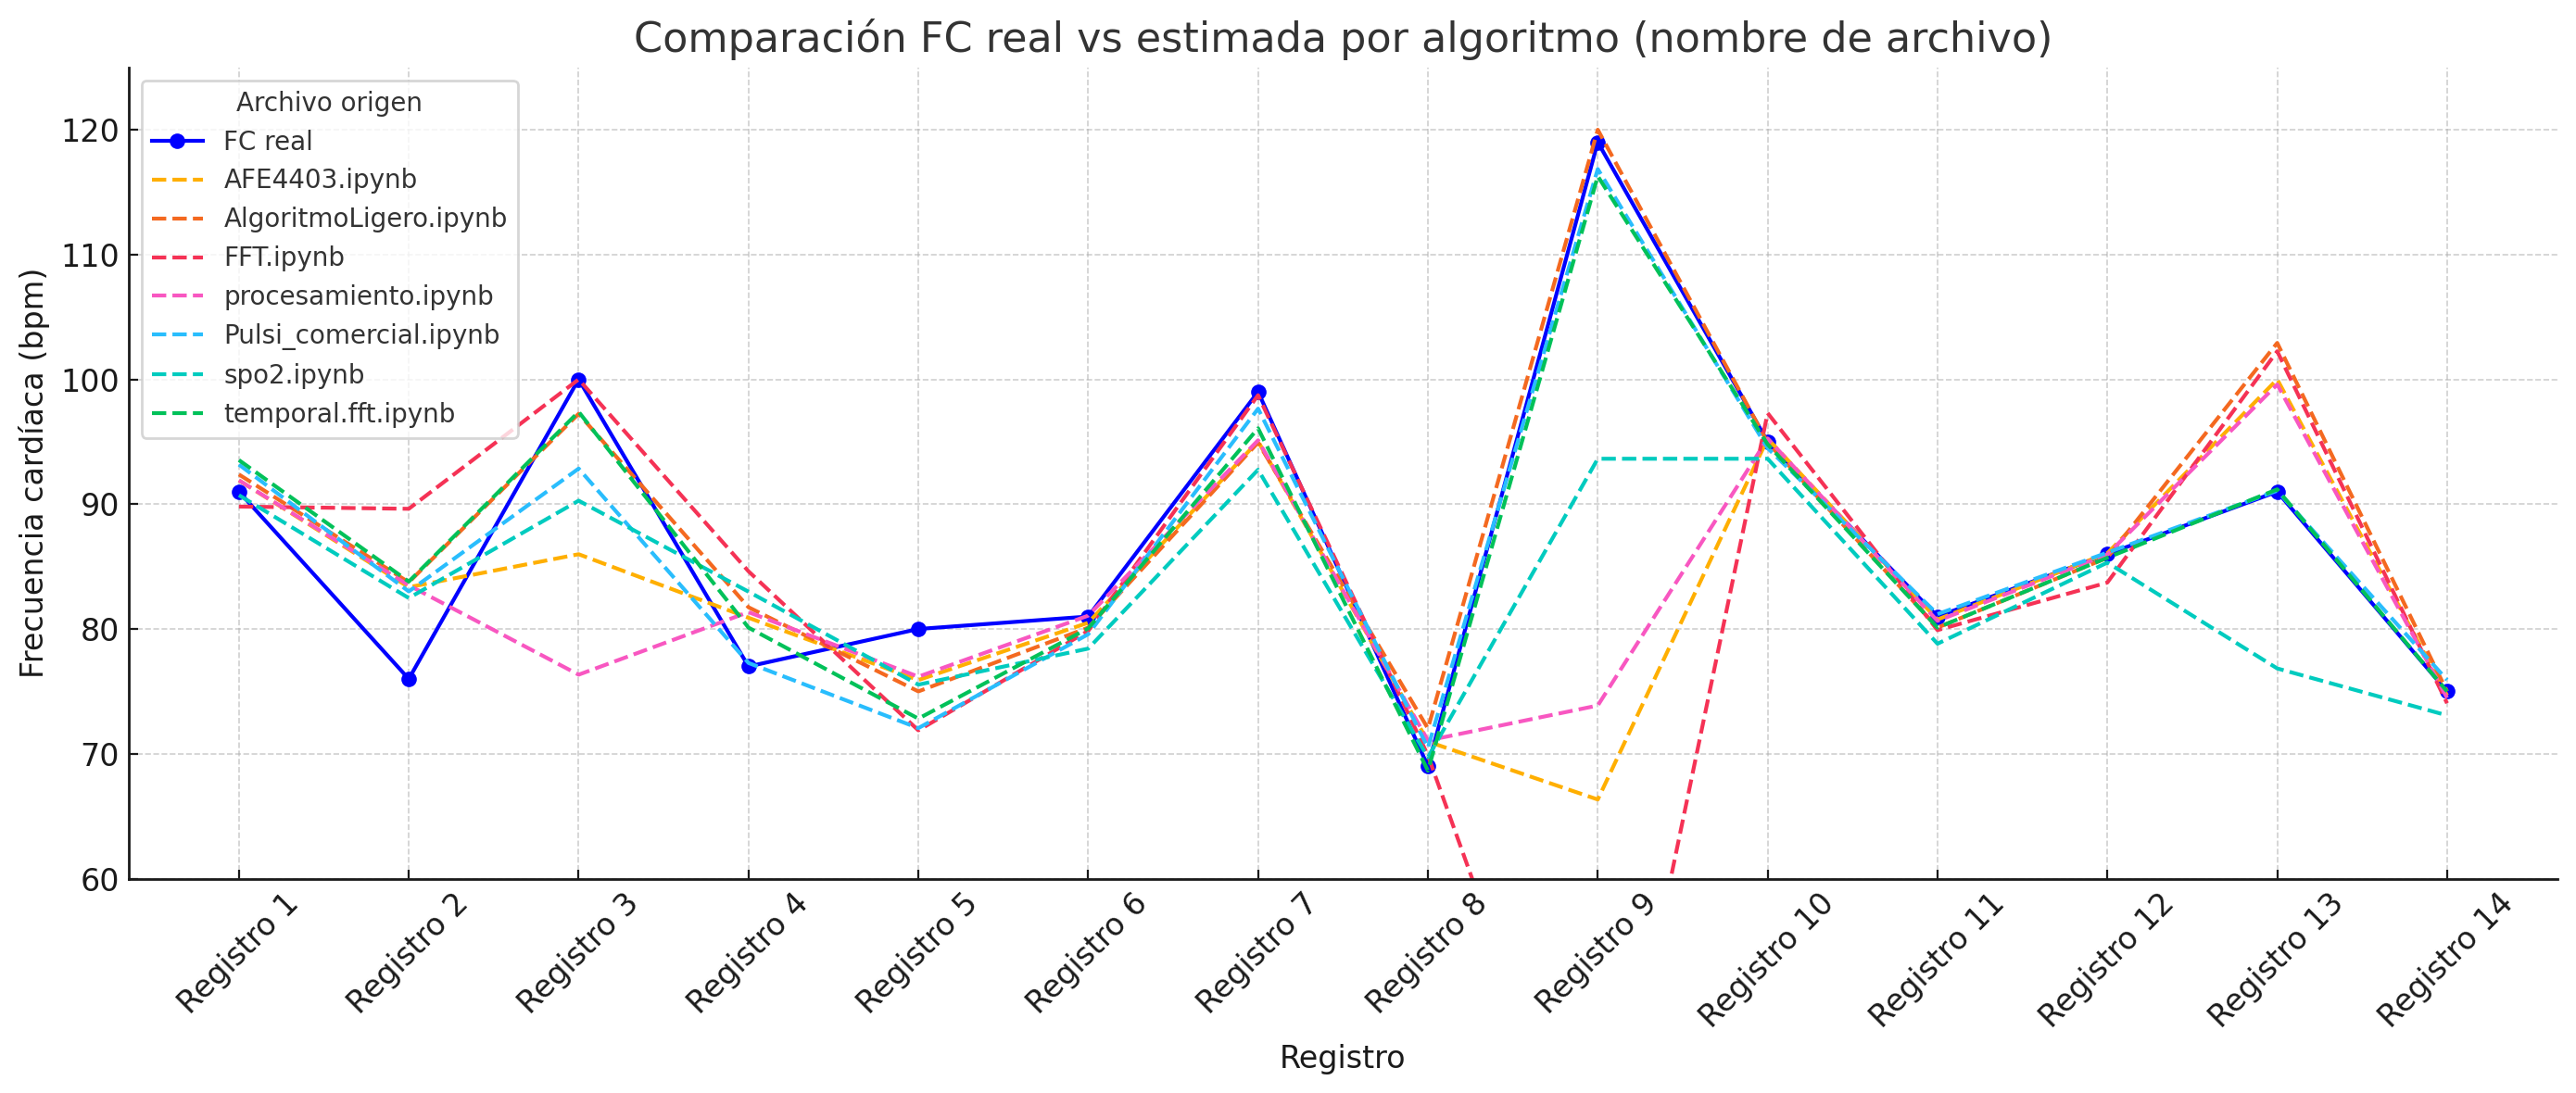
\includegraphics[width=1\linewidth]{img/calculo_fc.png}
    \caption{Gráfica comparativa entre entre la frecuencia cardíaca real y las frecuencias estimadas. \textit{Elaboración propia.}}
    \label{fig:comparacion_fc_algoritmos}
\end{figure}

A continuación se recogen los resultados detallados en forma tabular para cada uno de los métodos evaluados:


%\vspace{-1em} 

\begin{table}[H]
\centering
\begin{tabular}{|c|c|c|}
\hline
\textbf{FC esperada (bpm)} & \textbf{FC calculada (bpm)} & \textbf{Error relativo (\%)} \\
\hline
91 & 91.91 & 1.00 \\
\hline
76 & 83.35 & 9.67 \\
\hline
100 & 85.99 & 14.01 \\
\hline
77 & 80.90 & 5.06 \\
\hline
80 & 75.91 & 5.11 \\
\hline
81 & 80.50 & 0.62 \\
\hline
99 & 95.04 & 4.00 \\
\hline
106 & 77.17 & 27.20 \\
\hline
69 & 70.98 & 2.87 \\
\hline
119 & 66.34 & 44.25 \\
\hline
95 & 95.25 & 0.26 \\
\hline
81 & 80.76 & 0.30 \\
\hline
86 & 86.07 & 0.08 \\
\hline
91 & 100.00 & 9.89 \\
\hline
75 & 74.67 & 0.44 \\
\hline
91 & 82.55 & 9.29 \\
\hline
\end{tabular}
\caption{Error relativo (\%) entre FC esperada y calculada tras aplicar filtro Butterworth, correspondiente al archivo \texttt{AFE4403.ipynb.}}
\label{tabla:fc_afe4403_error_relativo}
\end{table}



\begin{table}[H]
\centering
\resizebox{\textwidth}{!}{%
\begin{tabular}{|c|c|c|c|c|}
\hline
\textbf{FC esperada (bpm)} & \textbf{HR IR (bpm)} & \textbf{HR RED (bpm)} & \textbf{Error IR (\%)} & \textbf{Error RED (\%)} \\
\hline
91 & 92.38 & 70.59 & 1.52 & 22.45 \\
\hline
76 & 83.74 & 82.87 & 10.18 & 9.04 \\
\hline
100 & 97.24 & 73.53 & 2.76 & 26.47 \\
\hline
77 & 81.74 & 80.11 & 6.16 & 4.04 \\
\hline
80 & 75.00 & 75.00 & 6.25 & 6.25 \\
\hline
81 & 80.11 & 80.11 & 1.10 & 1.10 \\
\hline
99 & 94.94 & 94.94 & 4.10 & 4.10 \\
\hline
106 & 100.08 & 94.94 & 5.59 & 10.53 \\
\hline
69 & 72.03 & 72.03 & 4.39 & 4.39 \\
\hline
119 & 120.00 & 120.24 & 0.84 & 1.04 \\
\hline
95 & 94.94 & 94.94 & 0.06 & 0.06 \\
\hline
81 & 80.11 & 80.11 & 1.10 & 1.10 \\
\hline
86 & 85.71 & 85.84 & 0.34 & 0.19 \\
\hline
91 & 102.92 & 102.92 & 13.09 & 13.09 \\
\hline
75 & 75.00 & 73.53 & 0.00 & 1.96 \\
\hline
91 & 81.86 & 66.67 & 10.06 & 26.75 \\
\hline
\end{tabular}%
}
\caption{Error relativo (\%) entre FC esperada y HR calculadas, correspondiente al archivo \texttt{AlgoritmoLigero.ipynb}.}
\label{tabla:fc_algoritmo_ligero_error_relativo}
\end{table}



\begin{table}[H]
\centering
\resizebox{\textwidth}{!}{%
\begin{tabular}{|c|c|c|}
\hline
\textbf{FC esperada (bpm)} & \textbf{FC estimada (bpm)} & \textbf{Error relativo (\%)} \\
\hline
91 & 89.81 & 1.31 \\
\hline
76 & 89.63 & 17.93 \\
\hline
100 & 100.00 & 0.00 \\
\hline
77 & 84.62 & 9.90 \\
\hline
80 & 71.88 & 10.15 \\
\hline
81 & 79.85 & 1.42 \\
\hline
99 & 98.73 & 0.27 \\
\hline
106 & 30.00 & 71.70 \\
\hline
69 & 69.87 & 1.26 \\
\hline
119 & 31.96 & 73.14 \\
\hline
95 & 97.30 & 2.42 \\
\hline
81 & 79.91 & 1.35 \\
\hline
86 & 83.72 & 2.65 \\
\hline
91 & 102.25 & 12.36 \\
\hline
75 & 74.05 & 1.27 \\
\hline
\end{tabular}%
}
\caption{Error relativo (\%) entre FC esperada y FC estimada tras representar la señal en forma FFT, correspondiente al archivo \texttt{FFT.ipynb.}}
\label{tabla:fc_fft_error_relativo}
\end{table}


\begin{table}[htbp]
\centering
\resizebox{\textwidth}{!}{%
\begin{tabular}{|c|c|c|}
\hline
\textbf{FC esperada (bpm)} & \textbf{FC estimada (bpm)} & \textbf{Error relativo (\%)} \\
\hline
91 & 91.91 & 1.00 \\
\hline
76 & 83.50 & 9.87 \\
\hline
100 & 76.34 & 23.66 \\
\hline
77 & 81.35 & 5.65 \\
\hline
80 & 76.18 & 4.77 \\
\hline
81 & 81.07 & 0.09 \\
\hline
99 & 95.12 & 3.92 \\
\hline
106 & 66.77 & 37.01 \\
\hline
69 & 71.07 & 3.00 \\
\hline
119 & 73.87 & 37.92 \\
\hline
95 & 95.25 & 0.26 \\
\hline
81 & 80.65 & 0.43 \\
\hline
86 & 85.97 & 0.03 \\
\hline
91 & 99.59 & 9.44 \\
\hline
75 & 74.48 & 0.69 \\
\hline
91 & 82.05 & 9.84 \\
\hline
\end{tabular}%
}
\caption{Error relativo (\%) entre FC esperada y FC estimada tras aplicar filtro Butterworth paso bajo y FFT, correspondiente al archivo \texttt{procesamiento.ipynb}.}
\label{tabla:fc_procesamiento_error_relativo}
\end{table}


\begin{table}[htbp]
\centering
\resizebox{\textwidth}{!}{%
\begin{tabular}{|c|c|c|}
\hline
\textbf{FC esperada (bpm)} & \textbf{FC estimada (bpm)} & \textbf{Error relativo (\%)} \\
\hline
91 & 93.17 & 2.38 \\
\hline
76 & 83.01 & 9.22 \\
\hline
100 & 92.85 & 7.15 \\
\hline
77 & 77.28 & 0.36 \\
\hline
80 & 72.06 & 9.92 \\
\hline
81 & 79.58 & 1.75 \\
\hline
99 & 97.65 & 1.36 \\
\hline
106 & 105.98 & 0.02 \\
\hline
69 & 70.49 & 2.16 \\
\hline
119 & 116.85 & 1.81 \\
\hline
95 & 94.49 & 0.54 \\
\hline
81 & 81.19 & 0.23 \\
\hline
86 & 86.12 & 0.14 \\
\hline
91 & 91.08 & 0.09 \\
\hline
75 & 75.92 & 1.23 \\
\hline
91 & 82.82 & 8.99 \\
\hline
\end{tabular}%
}
\caption{Error relativo (\%) entre FC esperada y FC estimada tras aplicar filtro Butterworth pasa-banda, correspondiente al archivo \texttt{Pulsi\_comercial.ipynb}}
\label{tabla:fc_pulsioximetro_comercial_error_relativo}
\end{table}


\begin{table}[H]
\centering
\resizebox{\textwidth}{!}{%
\begin{tabular}{|c|c|c|}
\hline
\textbf{FC esperada (bpm)} & \textbf{FC estimada (bpm)} & \textbf{Error relativo (\%)} \\
\hline
91 & 90.72 & 0.31 \\
\hline
76 & 82.48 & 8.53 \\
\hline
100 & 90.28 & 9.72 \\
\hline
77 & 82.99 & 7.78 \\
\hline
80 & 75.54 & 5.57 \\
\hline
81 & 78.43 & 3.17 \\
\hline
99 & 92.76 & 6.30 \\
\hline
69 & 69.72 & 1.04 \\
\hline
95 & 93.64 & 1.43 \\
\hline
81 & 78.82 & 2.69 \\
\hline
86 & 85.32 & 0.79 \\
\hline
75 & 73.08 & 2.56 \\
\hline
91 & 76.84 & 15.56 \\
\hline
\end{tabular}%
}
\caption{Error relativo (\%) entre FC esperada y FC estimada tras aplicar filtro de media y mediana, correspondiente al archivo \texttt{spo2.ipynb}.}
\label{tabla:fc_media_mediana_error_relativo}
\end{table}



\begin{table}[H]
\centering
\resizebox{\textwidth}{!}{%
\begin{tabular}{|c|c|c|}
\hline
\textbf{FC esperada (bpm)} & \textbf{FC estimada (bpm)} & \textbf{Error relativo (\%)} \\
\hline
91 & 93.53 & 2.78 \\
\hline
76 & 83.80 & 10.26 \\
\hline
100 & 97.40 & 2.60 \\
\hline
77 & 80.11 & 4.04 \\
\hline
80 & 72.82 & 8.98 \\
\hline
81 & 80.05 & 1.17 \\
\hline
99 & 96.08 & 2.95 \\
\hline
106 & 103.09 & 2.75 \\
\hline
69 & 68.65 & 0.51 \\
\hline
119 & 116.28 & 2.29 \\
\hline
95 & 94.79 & 0.22 \\
\hline
81 & 80.11 & 1.10 \\
\hline
86 & 85.71 & 0.34 \\
\hline
91 & 91.19 & 0.21 \\
\hline
75 & 75.00 & 0.00 \\
\hline
91 & 80.11 & 11.97 \\
\hline
\end{tabular}%
}
\caption{Estimación de frecuencia cardíaca con error relativo corregido, correspondiente al archivo \texttt{temporal\_fft.ipynb.}}
\label{tabla:fc_temporal_fft_error}
\end{table}



La frecuencia cardíaca estimada por los algoritmos aplicados tiene un error medio absoluto inferior a 5 BPM en la mayoría de los casos, lo que indica un comportamiento fiable.

Como se ha explicado en la metodología, el método que resultó más viable para ser implementado en el firmware fue el doble filtro de media móvil + mediana, por su optimización y simplicidad, además de ser uno de los procedimientos que mejores resultados obtiene.

\subsection{Resumen resultados de la estimación de la SpO$_2$ con Python}

A diferencia de la frecuencia cardíaca, la estimación de la SpO\textsubscript{2} ha resultado más complicada. Esto se debe a que su rango es más pequeño (normalmente entre 90 y 100\,\%) y cualquier pequeño error en las señales afecta mucho más al resultado final. Además, es un parámetro que depende de la relación entre dos señales (IR y RED), lo que lo hace más sensible a ruido o diferencias de amplitud.

Aunque en Python se han podido probar distintas fórmulas y enfoques, los resultados no han sido tan cercanos al valor real como los que se obtuvieron para la estimación de la frecuencia cardíaca (en la mayoría de los casos). Por este motivo, se trabajó directamente esta parte en el firmware, adaptando el algoritmo a las limitaciones reales del sistema, con el objetivo de asegurar una estimación fiable en tiempo real.

En las siguientes tablas se presentan los resultados obtenidos al aplicar diferentes métodos de estimación de la SpO\textsubscript{2} a los archivos de señal registrados durante el proyecto. Para cada uno de ellos se compara el valor estimado con el valor de referencia extraído del nombre del archivo.

Las estimaciones se han realizado utilizando los enfoques explicados en la sección \ref{cap: Metodología}: desde fórmulas empíricas, hasta métodos más simples como la regresión lineal o el uso de tablas LUT. También se ha incluido un cálculo del error asociado, cuando ha sido posible. Además, se ha intentado que quede más claro con gráficas que enfrentan los valores reales frente a los estimados por cada algoritmo.


\begin{table}[H]
\centering
\begin{tabular}{|c|c|c|}
\hline
\textbf{SpO\textsubscript{2} real (\%)} & \textbf{SpO\textsubscript{2} estimada (\%)} & \textbf{Error (\%)} \\
\hline
91 & 95 & 4 \\
\hline
92 & 95 & 3 \\
\hline
93 & 96 & 3 \\
\hline
95 & 97 & 2 \\
\hline
95 & 99 & 4 \\
\hline
95 & 98 & 3 \\
\hline
95 & 98 & 3 \\
\hline
96 & 96 & 0 \\
\hline
96 & 99 & 3 \\
\hline
97 & 0 & 97 \\
\hline
98 & 96 & 2 \\
\hline
98 & 90 & 8 \\
\hline
99 & 95 & 4 \\
\hline
99 & 97 & 2 \\
\hline
99 & 95 & 4 \\
\hline
\end{tabular}
\caption{Comparativa entre la SpO\textsubscript{2} esperada y estimada a partir de los archivos de señal. Archivo de referencia: \texttt{spo\_algo\_v4.ipynb.}}
\label{tabla:spo2_validacion_maxim}
\end{table}

\begin{figure}[H]
    \centering
    
\includegraphics[width=0.95\linewidth]{img/grafico_spo_algo_v4.png}
    \caption{Saturación esperada vs Saturación calculada. Archivo de referencia: \texttt{spo\_algo\_v4.ipynb.}}
    \label{fig:grafico_spo_algo_v4}
\end{figure}


\begin{table}[H]
\centering
\begin{tabular}{|c|c|c|}
\hline
\textbf{SpO\textsubscript{2} real (\%)} & \textbf{Ratio R} & \textbf{SpO\textsubscript{2} estimada (\%)} \\
\hline
91 & 0.000000 & 95.20 \\
\hline
92 & 8.099103 & 88.32 \\
\hline
93 & 0.000000 & 95.20 \\
\hline
95 & 2.484700 & 94.79 \\
\hline
95 & 2.403625 & 93.16 \\
\hline
95 & 0.561102 & 94.72 \\
\hline
95 & 1.543552 & 93.89 \\
\hline
96 & 0.745609 & 94.57 \\
\hline
96 & 1.046738 & 94.31 \\
\hline
97 & 0.617578 & 94.68 \\
\hline
97 & 13.812844 & 83.46 \\
\hline
98 & 2.875030 & 92.75 \\
\hline
98 & 12.062808 & 84.94 \\
\hline
98 & 1.424948 & 94.00 \\
\hline
99 & 2.470356 & 93.10 \\
\hline
99 & 0.000000 & 95.20 \\
\hline
\end{tabular}
\caption{Estimación de SpO\textsubscript{2} mediante fórmula lineal (95.20 - 0.85 · R).\\
Archivo de referencia: \texttt{tabla\_LUT.ipynb.}}

\label{tabla:spo2_formula_lineal}
\end{table}

\begin{figure}[H]
    \centering
    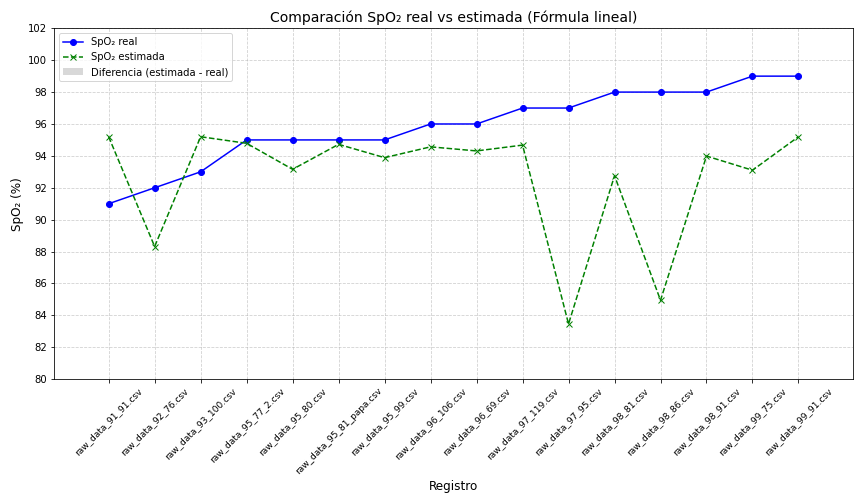
\includegraphics[width=0.95\linewidth]{img/grafico_tabla_LUT.png}
    \caption{Saturación esperada vs Saturación calculada. Archivo de referencia: Archivo de referencia: \texttt{tabla\_LUT.ipynb.}}
    \label{fig:grafico_spo2_lut}
\end{figure}


\begin{table}[H]
\centering
\begin{tabular}{|c|c|c|c|}
\hline
\textbf{SpO\textsubscript{2} real (\%)} & \textbf{SpO\textsubscript{2} estimado medio (\%)} & \textbf{Error (\%)} \\
\hline
91.0 & 95.26 & 4.26 \\
\hline
 92.0 & 96.74 & 4.74 \\
 \hline
93.0 & 96.72 & 3.72 \\
\hline
95.0 & 95.92 & 0.92 \\
\hline
95.0 & 96.36 & 1.36 \\
\hline
95.0 & 94.35 & 0.65 \\
\hline
 95.0 & 96.06 & 1.06 \\
 \hline
 96.0 & 95.97 & 0.03 \\
 \hline
96.0 & 95.89 & 0.11 \\
\hline
97.0 & 95.81 & 1.19 \\
\hline
97.0 & 96.79 & 0.21 \\
\hline
98.0 & 96.52 & 1.48 \\
\hline
98.0 & 96.78 & 1.22 \\
\hline
98.0 & 96.24 & 1.76 \\
\hline
99.0 & 95.35 & 2.65 \\
\hline
99.0 & 95.54 & 3.46 \\
\hline
\end{tabular}
\caption{Comparativa de SpO\textsubscript{2} real, estimación media y error medio. Archivo de referencia: \texttt{Paper\_CS.ipynb}}
\label{tabla:spo2_error_medio}
\end{table}

\begin{figure}[H]
    \centering
    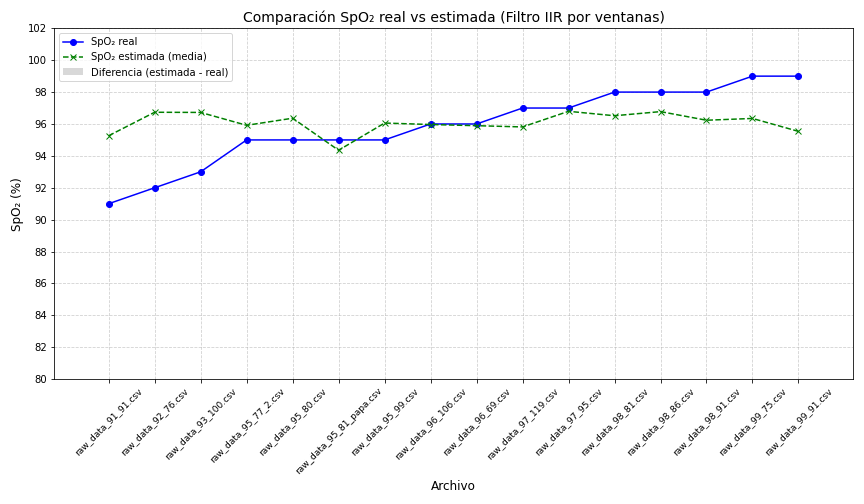
\includegraphics[width=0.95\linewidth]{img/grafico_Paper_CS.png}
    \caption{Saturación esperada vs Saturación calculada. Archivo de referencia: Archivo de referencia: \texttt{Paper\_CS.ipynb.}}
    \label{fig:grafico_Paper_CS}
\end{figure}


\begin{table}[H]
\centering
\begin{tabular}{|l|c|c|c|c|}
\hline
\textbf{SpO\textsubscript{2} real (\%)} & \textbf{Ratio R} & \textbf{SpO\textsubscript{2} estimada (\%)} & \textbf{Error (\%)} \\
\hline
91 & 0.117 & 91 & 0 \\
\hline
92 & 11.906 & 93 & 1 \\
\hline
95 & 0.816 & 77 & 18 \\
\hline
95 & 2.604 & 93 & 2 \\
\hline
95 & 0.538 & 95 & 0 \\
\hline
95 & 1.826 & 95 & 0 \\
\hline
96 & 0.957 & 93 & 3 \\
\hline
96 & 0.912 & 96 & 0 \\
\hline
97 & 0.695 & 97 & 0 \\
\hline
97 & 16.143 & 93 & 4 \\
\hline
98 & 4.252 & 93 & 5 \\
\hline
98 & 1.287 & 98 & 0 \\
\hline
99 & 2.312 & 93 & 6 \\
\hline
99 & 1.805 & 99 & 0 \\
\hline
\end{tabular}
\caption{Estimación de SpO\textsubscript{2} a partir del ratio R, extraída de los archivos de registro. Archivo de referencia: \texttt{uch\_spo2\_table.ipynb.}}
\label{tabla:spo2_ratio_r}
\end{table}

\begin{figure}[H]
    \centering
    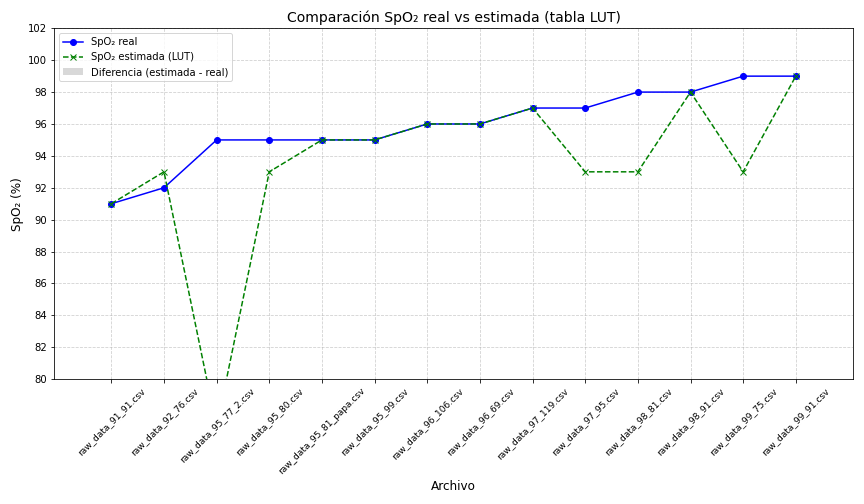
\includegraphics[width=0.95\linewidth]{img/grafico_spo2_lut.png}
    \caption{Saturación esperada vs Saturación calculada. Archivo de referencia: Archivo de referencia: \texttt{uch\_spo2\_tableipynb.}}
    \label{fig:grafico_spo2_lut}
\end{figure}

En el firmware se ha implementado un único algoritmo de estimación de SpO\textsubscript{2}, basado en el método del \textit{Ratio of Ratios} y el uso de una tabla LUT predefinida, que coincide con el implementado en el archivo \texttt{uch\_spo2\_table.ipynb}. Este enfoque fue seleccionado por su simplicidad computacional, bajo coste de recursos y facilidad de adaptación al entorno embebido.



\subsection{Resumen de los resultado de los algoritmos seleccionados en el firmware}

Integrados los algoritmos seleccionados en el firmware, el siguiente paso fue comprobar si realmente funcionaban como se esperaba al ejecutarse directamente sobre el microcontrolador\footnote{A diferencia de la metodología y resultados explicados en el entorno Python, que partían de los datos crudos en formato csv, el firmware recoge los datos que registra el sensor en tiempo real.}. En esta fase, el objetivo ya no es explicar cómo se ha hecho la adaptación (algo que ya se detalla en la metodología), sino observar el comportamiento del sistema en tiempo real y validar que los resultados obtenidos sean coherentes con los que se habían obtenido previamente en las pruebas realizadas en Python.

Para ello, se ejecutó el sistema completo en la placa y se observó la salida por consola, verificando que tanto la frecuencia cardíaca como la SpO\textsubscript{2} se estimaban de forma continua, sin bloqueos y con valores lo más parecidos posible a los mostrados por un pulsioxímetro de referencia con el que se mide al mismo tiempo. 

En la figura \ref{fig:firmware_resultados} se muestran ejemplos reales de la salida del sistema en funcionamiento. En cada línea se informa de la frecuencia cardíaca detectada y del valor de SpO\textsubscript{2} estimado. Como se puede apreciar, los valores se mantienen dentro de un rango fisiológicamente válido, y en muchos casos coinciden con los valores medidos manualmente mediante el sistema de referencia.

\begin{figure}[H]
\centering
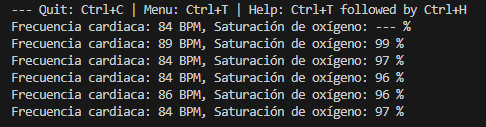
\includegraphics[width=0.8\textwidth]{img/Captura_firmware.png}
\caption{Salida por consola del firmware con los valores estimados de frecuencia cardíaca y SpO\textsubscript{2}. En ese momento se marcaba en el pulsioxímetro comercial un valor de 86 BPM y 98\% de SpO$_2$.}
\label{fig:firmware_resultados}
\end{figure}

En algunos casos puntuales se obtiene un valor de SpO\textsubscript{2} indicado como ``---'', lo cual se debe a que la señal en ese momento no cumplía con los criterios de validación definidos para evitar estimaciones erróneas. El sistema es muy sensible a la luz y al movimiento, como ya se ha mencionado a lo largo de la memoria; por ello, obtener mediciones válidas es complicado. También hay que tener en cuenta que en la mayoría de los casos, los valores indicados como ``---''se deben a que el sistema todavía tiene que estabilizarse.


Además de la captura mostrada, se ha grabado un breve vídeo \footnote{Disponible en el repositorio del proyecto, en el directorio de \texttt{Demostraciones.}} donde se puede ver en tiempo real cómo funciona el sistema al estar conectado a la placa. En él se muestra cómo, tras unos segundos de estabilización, el pulsioxímetro comienza a mostrar valores actualizados de frecuencia cardíaca y SpO \textsubscript{2} por la terminal de VSCode. Este vídeo tiene como objetivo ilustrar visualmente el funcionamiento final del sistema y demostrar que la estimación se realiza de forma continua, en tiempo real, y con una salida estable que responde a los datos recogidos por el sensor.

En conjunto, estos resultados indican que el sistema es capaz de estimar en tiempo real los parámetros fisiológicos de interés, y que los algoritmos seleccionados funcionan de forma coherente en el entorno embebido, respetando las limitaciones de recursos del microcontrolador y manteniéndose dentro de un margen razonable de precisión.


\section{Discusión.}

El resultado final del sistema es una salida en tiempo real que muestra por consola los valores estimados de frecuencia cardíaca y saturación de oxígeno. Como se puede ver en la figura \ref{fig:firmware_resultados}, el sistema es capaz de ofrecer estos datos de manera continua y estable, con valores que entran dentro de los rangos fisiológicamente esperados y que, en la mayoría de los casos, se aproximan bastante a los mostrados por un pulsioxímetro comercial usado como referencia.

Este comportamiento confirma que el sistema no solo es capaz de adquirir y procesar señales reales fsin necesidad de recurrir a procesamiento posterior en un ordenador. A nivel práctico, esto implica que el pulsioxímetro se podría usar directamente en la incubadora, sin depender de equipamiento adicional.

En los entornos hospitalarios avanzados, las incubadoras no suelen integrar el pulsioxímetro como parte del sistema base. Lo habitual es que se conecte un monitor multiparamétrico externo, que incluye otros sensores además del de SpO\textsubscript{2}, y que se coloca al neonato mediante una pinza o parche adhesivo. En cambio, la solución desarrollada en este proyecto está pensada para estar integrada físicamente en la incubadora \textit{In$^3$ator}, y mostrar sus valores de forma conjunta con otros parámetros que ya se controlaban anteriormente, como la temperatura o la humedad. 

Respecto a la comparación con sistemas existentes, es evidente que el prototipo desarrollado no puede competir con la precisión ni la estabilidad de pulsioxímetros comerciales o sistemas que actualmente se emplean en entornos para los que está pensado el trabajo. Sin embargo, eso no quita que se puedan sacar conclusiones interesantes sobre su rendimiento, sobre todo si lo comparamos con otros prototipos más parecidos en objetivos y contexto.

La mayoría de los proyectos mencionados en la sección de conceptos teóricos se centran en fases previas al uso embebido: analizan señales offline, simulan el comportamiento de los sensores o muestran gráficas en Matlab o Python. Por ejemplo, el trabajo de Olga Jiménez\cite{jimenez2019pulsioximetro} desarrolla una interfaz gráfica para la monitorización de constantes, pero el procesado no se integra en un sistema físico. De forma parecida, en el proyecto de Francisco González Romero\cite{gonzalez2019pulsioximetro}, en el que se trabaja con adquisición de señales reales y análisis en entorno PC, pero no se llega a integrar el sistema completo en firmware.

En el caso del trabajo de Jorge Alarcó, de la Universidad Politécnica de Madrid \cite{Alarco2015} sí se llega a validar un sistema real, pero su objetivo está más centrado en la comparación de exactitud frente a modelos certificados, y no en la integración funcional en un entorno concreto como una incubadora.

En cambio, este proyecto ha apostado por una solución pensada para incorporarse desde el diseño al producto final. Esto implica tener en cuenta no solo el rendimiento técnico del algoritmo, sino también la facilidad de fabricación, consumo de recursos y fiabilidad del funcionamiento. El hecho de que los valores de frecuencia cardíaca y SpO\textsubscript{2} se puedan calcular, filtrar y mostrar directamente en pantalla, usando únicamente el microcontrolador y un sensor óptico, supone un paso importante hacia una solución más autónoma y accesible.


